\chapter{Weerstandsschatting en aandrijflijn}
\label{ch:holtrop-aandrijflijn}

\noindent In dit hoofdstuk wordt deelvraag 2 beantwoord:

\begin{quote}
    \textit{\textbf{Welk energieopslagsysteem past het best bij Jansje, gegeven de
    technische parameters, het operationele profiel en de financiële parameters?}}
\end{quote}

\noindent Hiervoor is het benodigd aandrijfvermogen een belangrijke
invoerparameter. Om deze te verkrijgen, wordt eerst de scheepsweerstand geschat via de
Holtrop-Mennen methode. Daarna wordt de volledige aandrijflijn doorgerekend naar
het minimaal te installeren motorvermogen.

% ============================================================
\section{Weerstandsschatting met de Holtrop-Mennen methode}
\label{sec:holtrop}

De totale weerstand van \emph{'t~Jansje} in varende conditie is bepaald met de
statistische regressiemethode van Holtrop en Mennen \cite{Holtrop1984}. De methode
gaat uit van diepwater bij zeewater ($\rho = 1025\ \mathrm{kg/m^3}$,
$15\,^{\circ}\mathrm{C}$) en kalm water. Omdat \emph{'t~Jansje} op binnenwateren
vaart levert dit een conservatieve schatting; de bijbehorende beperkingen worden
behandeld in Sectie~\ref{subsec:holtrop-validatie}.

De totale weerstand is opgebouwd uit de volgende componenten \cite{Holtrop1984}:

\begin{equation}
    R_\mathrm{totaal} = R_F(1+k_1) + R_{APP} + R_W + R_B + R_{TR} + R_A
    \label{eq:Rtot}
\end{equation}

\noindent waarbij $R_F$ de wrijvingsweerstand is volgens de ITTC-1957 formulering,
$(1+k_1)$ de visceuze vormfactor van de romp, $R_{APP}$ de aanhangselweerstand,
$R_W$ de golfweerstand, $R_B$ en $R_{TR}$ resp.\ boegbulb- en spiegelweerstand,
en $R_A$ de modelschaalkorrelatieallowance. De wrijvingsweerstand volgt uit:

\begin{equation}
    R_F = \tfrac{1}{2}\,\rho\,V^2\,S\,C_F, \qquad
    C_F = \frac{0{,}075}{(\log Re - 2)^2}
    \label{eq:RF}
\end{equation}

De overige componenten worden berekend via regressieformules in de scheepsparameters
$L_{wl}$, $B$, $T$, $C_B$, $C_P$, $C_{WP}$, $C_M$ en $L_{CB}$; de volledige
uitwerking is geïmplementeerd in de spreadsheet \cite{spreadsheet_holtrop}.

% ------------------------------------------------------------------
\subsection{Scheepsgegevens}
\label{subsec:holtrop-scheepsgegevens}

\begin{table}[H]
\centering
\caption{Invoerparameters Holtrop-schatting, \emph{'t~Jansje} (varende conditie)}
\label{tab:holtrop_input}
\begin{tabular}{llll}
\toprule
Parameter & Symbool & Waarde & Eenheid \\
\midrule
Lengte waterlijn            & $L_{wl}$    & 22{,}22 & m        \\
Breedte waterlijn           & $B$         &  4{,}36 & m        \\
Diepgang voor- en achterschip & $T$       &  1{,}50 & m        \\
Verdringingsvolume          & $\nabla$    & 73{,}0  & m$^3$    \\
Hoofdspantcoëfficiënt       & $C_M$       &  0{,}90 & --       \\
Waterplancoëfficiënt        & $C_{WP}$    &  0{,}795& --       \\
Blokcoëfficiënt             & $C_B$       &  0{,}502& --       \\
Prismatische coëfficiënt    & $C_P$       &  0{,}558& --       \\
Halve instroomhoek          & $i_E$       & 17      & $^\circ$ \\
LCB-positie (t.o.v.\ $\tfrac{1}{2}L_{wl}$) & $LCB$\% & 0{,}0 & \% \\
Spiegeloppervlak            & $A_T$       & 0       & m$^2$    \\
Transversaal boegbulboppervlak & $A_{BT}$ & 0       & m$^2$    \\
Sternvormcoëfficiënt        & $C_{stern}$ & 0       & --       \\
Ruwheidsmaatstaf            & $k_s$       & 150     & $\mu$m   \\
\bottomrule
\end{tabular}
\end{table}

De regressieformules gelden alleen binnen een bepaalde range. Buiten die
range zijn de uitkomsten onbetrouwbaar. De Holltrop en Mennen spreadsheet
\cite{spreadsheet_holtrop} controleert dit automatisch.
Tabel~\ref{tab:holtrop_checks} toont de geldigheidscontroles voor \emph{'t~Jansje}.

\begin{table}[H]
\centering
\caption{Geldigheidscontroles Holtrop (1984) voor \emph{'t~Jansje}}
\label{tab:holtrop_checks}
\begin{tabular}{llcc}
\toprule
Parameter & Voorwaarde & Waarde & Geslaagd \\
\midrule
Lengte-breedte verhouding   & $3{,}9 \leq L_{wl}/B \leq 14{,}9$    & 5{,}10     & \cmark \\
Breedte-diepgang verhouding & $2{,}1 \leq B/T \leq 4{,}0$           & 2{,}91     & \cmark \\
Prismatische coëfficiënt    & $0{,}55 \leq C_P \leq 0{,}85$         & 0{,}558    & \cmark \\
LCB-positie                 & $-5\% \leq LCB\% \leq +5\%$           & 0{,}0\%    & \cmark \\
Halve instroomhoek          & $1^\circ \leq i_E \leq 90^\circ$      & $17^\circ$ & \cmark \\
Hoogte boegbulb boven kiel  & $0 \leq h_B \leq 0{,}6\,T$            & 0          & \cmark \\
Golfweerstandsparameter     & $0{,}01 \leq \lambda \leq 1{,}07$     & 0{,}654    & \cmark \\
Froude-getal (bij 7~kn)     & $F_n \leq 0{,}77$                     & 0{,}244    & \cmark \\
\bottomrule
\end{tabular}
\end{table}

Alle parameters vallen ruim binnen de geldigheidsrange bij de ontwerpsnelheid van
7~knopen:
\begin{equation}
    F_n = \frac{V}{\sqrt{g\,L_{wl}}}
        = \frac{3{,}601}{\sqrt{9{,}81 \times 22{,}22}}
        = 0{,}244
\end{equation}

% ------------------------------------------------------------------
\subsection{Afgeleide grootheden}
\label{subsec:holtrop-afgeleid}

\begin{table}[H]
\centering
\caption{Berekende grootheden op basis van de scheepsgeometrische invoer
         \cite{spreadsheet_holtrop}}
\label{tab:holtrop_derived}
\begin{tabular}{llll}
\toprule
Grootheid & Symbool & Waarde & Eenheid \\
\midrule
Vormfactor          & $(1+k_1)$    & 1{,}208                & --   \\
Nat oppervlak       & $S$          & 108{,}82               & m$^2$\\
Looplengte          & $L_R$        &   9{,}82               & m    \\
Correlatie-allowance& $C_A$        & $7{,}31 \times 10^{-4}$& --   \\
\bottomrule
\end{tabular}
\end{table}

De vormfactor $(1+k_1) = 1{,}208$ geeft aan dat de visceuze weerstand van de romp
ruim 20\% hoger ligt dan de vlakke-plaatswrijving; dit is karakteristiek voor een
relatief vol en kort schip met $C_B \approx 0{,}50$.

% ------------------------------------------------------------------
\subsection{Resultaten}
\label{subsec:holtrop-resultaten}

Bij de ontwerpsnelheid van 7~knoop ($V = 3{,}601\ \mathrm{m/s}$, $F_n = 0{,}244$)
levert de Holtrop-methode de weerstandscomponenten van
Tabel~\ref{tab:holtrop_results_7kn}.

\begin{table}[H]
\centering
\caption{Weerstandscomponenten bij $V = 7\ \mathrm{kn}$}
\label{tab:holtrop_results_7kn}
\begin{tabular}{lrr}
\toprule
Component & Waarde [kN] & Aandeel [\%] \\
\midrule
Wrijvingsweerstand (incl.\ vormfactor) $R_F(1+k_1)$ & 1{,}931 & 65{,}4 \\
Golfweerstand $R_W$                                   & 0{,}455 & 15{,}4 \\
Correlatie-allowance $R_A$                            & 0{,}529 & 17{,}9 \\
Aanhangselweerstand $R_{APP}$                         & 0{,}039 &  1{,}3 \\
Spiegelweerstand $R_{TR}$                             & 0       &  0{,}0 \\
Boegbulbweerstand $R_B$                               & 0       &  0{,}0 \\
\midrule
\textbf{Totale weerstand} $R_\mathrm{totaal}$
    & \textbf{2{,}953} & \textbf{100{,}0} \\
\midrule
Effectief vermogen $P_E = R_\mathrm{tot} \times V$
    & \multicolumn{2}{c}{$10{,}6\ \mathrm{kW}$} \\
\bottomrule
\end{tabular}
\end{table}

Het grote aandeel van de wrijvingsweerstand (65{,}4\%) is te verwachten bij het lage
Froude-getal van een binnenvaartschip. De golfweerstand is bij 7~knopen nog beperkt
(15{,}4\%), maar neemt snel toe bij hogere snelheden, zoals te zien in
Tabel~\ref{tab:holtrop_speed_series}.

\begin{table}[H]
\centering
\caption{Weerstand en effectief vermogen als functie van de snelheid
         \cite{spreadsheet_holtrop}}
\label{tab:holtrop_speed_series}
\begin{tabular}{rrrrrrr}
\toprule
$V$ [kn] & $V$ [m/s] & $F_n$ & $R_F(1{+}k_1)$ [kN] & $R_W$ [kN] & $R_A$ [kN]
         & $P_E$ [kW] \\
\midrule
6{,}0 & 3{,}087 & 0{,}209 & 1{,}452 & 0{,}123 & 0{,}389 &  6{,}15 \\
6{,}5 & 3{,}344 & 0{,}226 & 1{,}683 & 0{,}246 & 0{,}456 &  8{,}09 \\
\rowcolor{green!15}
7{,}0 & 3{,}601 & 0{,}244 & 1{,}931 & 0{,}455 & 0{,}529 & 10{,}63 \\
7{,}5 & 3{,}858 & 0{,}261 & 2{,}194 & 0{,}803 & 0{,}607 & 14{,}07 \\
8{,}0 & 4{,}116 & 0{,}279 & 2{,}472 & 1{,}276 & 0{,}691 & 18{,}47 \\
\bottomrule
\end{tabular}
\end{table}

% ------------------------------------------------------------------
\subsection{Operationele snelheidskeuze: 7~knoop}
\label{subsec:snelheidskeuze}

Uit gesprekken met eigenaar Wim van Baalen blijkt dat \emph{'t~Jansje} in de
praktijk op 6 à 7~knopen wordt gevaren \cite{vanbaalen2026interview}.

Bij 7~knoop is de golfweerstand al merkbaar hoger dan bij lagere snelheden:
$R_W$ stijgt van 0{,}12~kN bij 6~kn naar 0{,}46~kN bij 7~kn (factor~3{,}7).
Boven 7~knoop neemt de stijging verder toe; bij 8~kn is het effectief vermogen
74\% hoger dan bij 7~kn (18{,}5~kW vs.\ 10{,}6~kW), zonder dat je er echt een
tijdsvoordeel mee opdoet op de korte trajecten op de Nieuwe Maas.

Voor de dimensionering van aandrijflijn en energieopslag wordt \textbf{7~knopen}
aangehouden als \emph{maximum ontwerpsnelheid} en 6{,}5~knopen als
\emph{nominale kruissnelheid}.

% ------------------------------------------------------------------
\subsection{Figuren}
\label{subsec:holtrop-figuren}

Figuur~\ref{fig:holtrop_rtot} toont de totale weerstand als functie van de snelheid.
Figuur~\ref{fig:holtrop_stacked} geeft de opbouw van de weerstand in drie componenten.
Figuur~\ref{fig:holtrop_ehp} toont het effectief vermogen.
Figuur~\ref{fig:holtrop_pie} geeft de procentuele verdeling bij 7~knoop.

\begin{figure}[H]
\centering
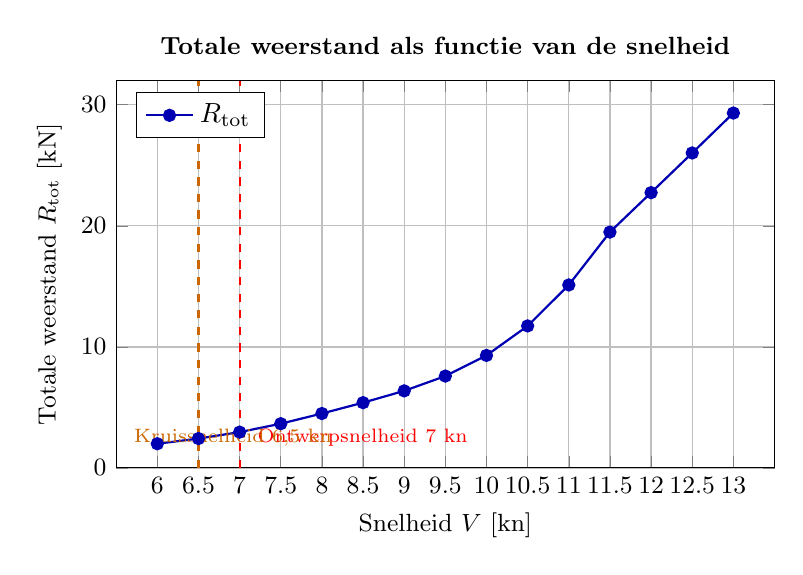
\begin{tikzpicture}
\begin{axis}[
    width=0.82\textwidth, height=6.5cm,
    xlabel={Snelheid $V$ [kn]},
    ylabel={Totale weerstand $R_\mathrm{tot}$ [kN]},
    title={Totale weerstand als functie van de snelheid},
    xmin=5.5, xmax=13.5, ymin=0, ymax=32,
    xtick={6,6.5,7,7.5,8,8.5,9,9.5,10,10.5,11,11.5,12,12.5,13},
    grid=both,
    grid style={line width=0.3pt, draw=gray!30},
    major grid style={line width=0.5pt, draw=gray!50},
    legend pos=north west,
    tick label style={font=\small},
    label style={font=\small},
    title style={font=\small\bfseries},
]
\addplot[blue!70!black, thick, mark=*, mark size=2pt] coordinates {
    (6.0,1.992)(6.5,2.419)(7.0,2.953)(7.5,3.648)(8.0,4.489)
    (8.5,5.386)(9.0,6.361)(9.5,7.584)(10.0,9.290)
    (10.5,11.727)(11.0,15.112)(11.5,19.482)(12.0,22.740)
    (12.5,26.018)(13.0,29.316)
};
\addlegendentry{$R_\mathrm{tot}$}
\addplot[red, dashed, thick, forget plot] coordinates {(7,0)(7,32)};
\addplot[orange!80!black, dashed, thick, forget plot] coordinates {(6.5,0)(6.5,32)};
\node[red, font=\scriptsize, anchor=south west]
    at (axis cs:7.1,1) {Ontwerpsnelheid 7~kn};
\node[orange!80!black, font=\scriptsize, anchor=south west]
    at (axis cs:5.6,1) {Kruissnelheid 6{,}5~kn};
\end{axis}
\end{tikzpicture}
\caption{Totale weerstand van \emph{'t~Jansje} als functie van de snelheid \cite{Holtrop1984, spreadsheet_holtrop}. Uit de grafiek is goed op te maken dat de golfweerstand significant toeneemt rond $F_n \approx 0{,}30$--$0{,}35$.}
\label{fig:holtrop_rtot}
\end{figure}

\begin{figure}[H]
\centering
\begin{tikzpicture}
\begin{axis}[
    width=0.82\textwidth, height=6.5cm,
    xlabel={Snelheid $V$ [kn]},
    ylabel={Weerstand [kN]},
    title={Weerstandscomponenten (gestapeld, 6--10~kn)},
    xmin=5.5, xmax=10.5, ymin=0, ymax=11,
    xtick={6,6.5,7,7.5,8,8.5,9,9.5,10},
    grid=both,
    grid style={line width=0.3pt, draw=gray!30},
    major grid style={line width=0.5pt, draw=gray!50},
    legend pos=north west, legend style={font=\small},
    tick label style={font=\small}, label style={font=\small},
    title style={font=\small\bfseries},
]
\addplot[name path=zero, draw=none, forget plot]
    coordinates {(6,0)(6.5,0)(7,0)(7.5,0)(8,0)(8.5,0)(9,0)(9.5,0)(10,0)};
\addplot[name path=RF, draw=none, forget plot] coordinates {
    (6,1.452)(6.5,1.683)(7,1.931)(7.5,2.194)(8,2.472)
    (8.5,2.766)(9,3.075)(9.5,3.399)(10,3.739)};
\addplot[name path=RFRW, draw=none, forget plot] coordinates {
    (6,1.575)(6.5,1.929)(7,2.386)(7.5,2.997)(8,3.748)
    (8.5,4.551)(9,5.426)(9.5,6.542)(10,8.136)};
\addplot[name path=RFRWRA, draw=none, forget plot] coordinates {
    (6,1.992)(6.5,2.419)(7,2.953)(7.5,3.648)(8,4.489)
    (8.5,5.386)(9,6.361)(9.5,7.584)(10,9.290)};
\addplot[fill=blue!40, fill opacity=0.75, draw=none, area legend]
    fill between[of=RF and zero];
\addlegendentry{$R_F(1{+}k_1)$}
\addplot[fill=red!45, fill opacity=0.75, draw=none, area legend]
    fill between[of=RFRW and RF];
\addlegendentry{$R_W$}
\addplot[fill=yellow!60, fill opacity=0.85, draw=none, area legend]
    fill between[of=RFRWRA and RFRW];
\addlegendentry{$R_A$}
\addplot[red, dashed, thick, forget plot] coordinates {(7,0)(7,11)};
\addplot[orange!80!black, dashed, thick, forget plot] coordinates {(6.5,0)(6.5,11)};
\end{axis}
\end{tikzpicture}
\caption{Gestapelde weerstandscomponenten voor \emph{'t~Jansje} in het bereik
         6--10~knoop. $R_W$ neemt sterk toe boven 7~knoop, terwijl
         $R_F(1+k_1)$ bij lage snelheden domineert. Rode stippellijn:
         ontwerpsnelheid; oranje stippellijn: kruissnelheid.}
\label{fig:holtrop_stacked}
\end{figure}

\begin{figure}[H]
\centering
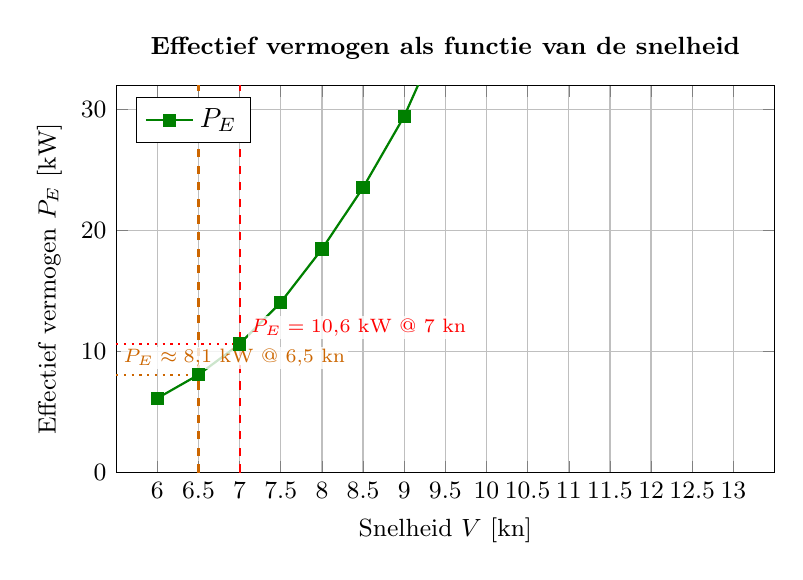
\begin{tikzpicture}
\begin{axis}[
    width=0.82\textwidth, height=6.5cm,
    xlabel={Snelheid $V$ [kn]},
    ylabel={Effectief vermogen $P_E$ [kW]},
    title={Effectief vermogen als functie van de snelheid},
    xmin=5.5, xmax=13.5, ymin=0, ymax=32,
    xtick={6,6.5,7,7.5,8,8.5,9,9.5,10,10.5,11,11.5,12,12.5,13},
    grid=both,
    grid style={line width=0.3pt, draw=gray!30},
    major grid style={line width=0.5pt, draw=gray!50},
    legend pos=north west,
    tick label style={font=\small}, label style={font=\small},
    title style={font=\small\bfseries},
]
\addplot[green!50!black, thick, mark=square*, mark size=2pt] coordinates {
    (6.0,6.150)(6.5,8.089)(7.0,10.633)(7.5,14.075)(8.0,18.472)
    (8.5,23.554)(9.0,29.451)(9.5,37.079)(10.0,47.784)
    (10.5,63.378)(11.0,85.596)(11.5,115.182)(12.0,140.308)
    (12.5,167.278)(13.0,195.991)
};
\addlegendentry{$P_E$}
\addplot[red, dashed, thick, forget plot] coordinates {(7,0)(7,32)};
\addplot[red, dotted, thick, forget plot] coordinates {(5.5,10.633)(7,10.633)};
\node[red, font=\scriptsize, anchor=south west,
      fill=white, fill opacity=0.8, text opacity=1, inner sep=1pt]
    at (axis cs:7.1,11) {$P_E = 10{,}6$~kW @ 7~kn};
\addplot[orange!80!black, dashed, thick, forget plot] coordinates {(6.5,0)(6.5,32)};
\addplot[orange!80!black, dotted, thick, forget plot] coordinates {(5.5,8.089)(6.5,8.089)};
\node[orange!80!black, font=\scriptsize, anchor=south west,
      fill=white, fill opacity=0.8, text opacity=1, inner sep=1pt]
    at (axis cs:5.55,8.5) {$P_E \approx 8{,}1$~kW @ 6{,}5~kn};
\end{axis}
\end{tikzpicture}
\caption{Effectief vermogen van \emph{'t~Jansje} als functie van de snelheid.
         Bij 7~knoop bedraagt $P_E = 10{,}6\ \mathrm{kW}$; de kruissnelheid
         van 6{,}5~kn vergt slechts $\approx 8{,}1\ \mathrm{kW}$.}
\label{fig:holtrop_ehp}
\end{figure}

\begin{figure}[H]
\centering
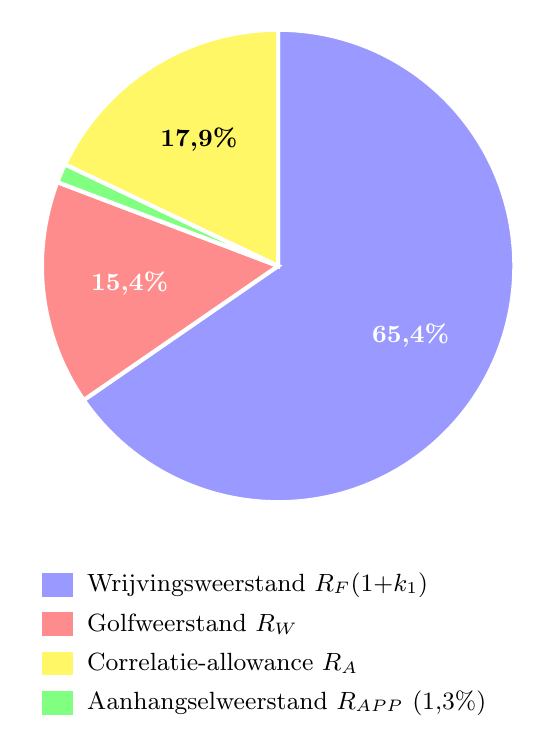
\begin{tikzpicture}
\def\R{3.0cm}
\fill[blue!40, draw=white, line width=1.5pt]
    (0,0) -- ({cos(90)*\R},{sin(90)*\R})
    arc[start angle=90, end angle=-145.4, radius=\R] -- cycle;
\fill[red!45, draw=white, line width=1.5pt]
    (0,0) -- ({cos(-145.4)*\R},{sin(-145.4)*\R})
    arc[start angle=-145.4, end angle=-200.8, radius=\R] -- cycle;
\fill[green!50, draw=white, line width=1.5pt]
    (0,0) -- ({cos(-200.8)*\R},{sin(-200.8)*\R})
    arc[start angle=-200.8, end angle=-205.5, radius=\R] -- cycle;
\fill[yellow!60, draw=white, line width=1.5pt]
    (0,0) -- ({cos(-205.5)*\R},{sin(-205.5)*\R})
    arc[start angle=-205.5, end angle=-270, radius=\R] -- cycle;
\node[font=\small\bfseries, white]
    at ({cos(-27.7)*1.9cm},{sin(-27.7)*1.9cm}) {65{,}4\%};
\node[font=\small\bfseries, white]
    at ({cos(-173.1)*1.9cm},{sin(-173.1)*1.9cm}) {15{,}4\%};
\node[font=\small\bfseries]
    at ({cos(-238)*1.9cm},{sin(-238)*1.9cm}) {17{,}9\%};
\fill[blue!40]  (-3.0,-4.2) rectangle (-2.6,-3.9);
\node[right, font=\small] at (-2.55,-4.05) {Wrijvingsweerstand $R_F(1{+}k_1)$};
\fill[red!45]   (-3.0,-4.7) rectangle (-2.6,-4.4);
\node[right, font=\small] at (-2.55,-4.55) {Golfweerstand $R_W$};
\fill[yellow!60](-3.0,-5.2) rectangle (-2.6,-4.9);
\node[right, font=\small] at (-2.55,-5.05) {Correlatie-allowance $R_A$};
\fill[green!50] (-3.0,-5.7) rectangle (-2.6,-5.4);
\node[right, font=\small] at (-2.55,-5.55) {Aanhangselweerstand $R_{APP}$ (1{,}3\%)};
\end{tikzpicture}
\caption{Procentuele verdeling van de weerstandscomponenten bij 7~knoop
         ($R_\mathrm{tot} = 2{,}95\ \mathrm{kN}$, $F_n = 0{,}244$).}
\label{fig:holtrop_pie}
\end{figure}

% ------------------------------------------------------------------
\subsection{Validatie en beperkingen}
\label{subsec:holtrop-validatie}

De Holtrop-Mennen methode is een statistische regressiemethode die
geschikt is voor vroege ontwerpfasen \cite{Holtrop1984}. De methode
geeft geen garantie op een specifieke nauwkeurigheid, want dat hangt
af van hoe goed het schip lijkt op de dataset waarop de regressie
gebaseerd is. Voor \emph{'t~Jansje} zijn drie kanttekeningen van belang:

\begin{itemize}
    \item \textbf{Aanhangsels:} $R_{APP}$ is gebaseerd op een schatting van het
          natte roeroppervlak achter een skeg. Bij definitieve vaststelling van
          het aandrijfconcept dient dit nader te worden bepaald.

    \item \textbf{Ondiepwater-effect:} De methode is ontwikkeld voor diepwater.
          Het vaargebied (Nieuwe Maas, Maassluis) heeft een waterdiepte van
          5--10~m, wat bij een diepgang van 1{,}50~m een verhouding
          $h/T \approx 3$--$7$ oplevert. Bij $h/T < 4$ treden
          ondiepwatereffecten op.

    \item \textbf{Golven en wind:} De berekening geldt voor kalm water. Marges
          voor golfweerstand en windweerstand zijn toegevoegd in de
          20\%-marge uit Sectie~\ref{subsec:aandrijflijn-berekening}.
\end{itemize}

Het resultaat ($P_E = 10{,}6\ \mathrm{kW}$ bij 7~knopen) vormt de invoer voor
de aandrijflijnanalyse in de volgende sectie.

% ============================================================
\section{Doorrekening aandrijflijn}
\label{sec:aandrijflijn}

Met het effectief trekvermogen $P_E$ bekend, wordt de volledige aandrijflijn
doorgerekend om het minimaal te installeren motorvermogen $P_B$ te bepalen.

% ------------------------------------------------------------------
\subsection{Aandrijflijnsketen}
\label{subsec:propulsion-chain}

Figuur~\ref{fig:propulsion-chain} toont de aandrijflijnsketen van
scheepsweerstand tot energiebron \cite{Molland2011}.

\begin{figure}[H]
\centering
\begin{tikzpicture}[
    node distance=1.1cm and 1.6cm,
    box/.style={rectangle, draw=blue!60!black, fill=blue!8,
                rounded corners=3pt, text width=3.0cm,
                align=center, font=\small, inner sep=5pt, minimum height=1.2cm},
    eff/.style={rectangle, draw=orange!70!black, fill=orange!12,
                rounded corners=2pt, text width=2.4cm,
                align=center, font=\scriptsize, inner sep=4pt, minimum height=0.9cm},
    arr/.style={-{Stealth[length=6pt]}, thick, blue!60!black},
    effArr/.style={-{Stealth[length=5pt]}, thick, dashed, orange!70!black},
]
\node[box] (PE)  {Effectief trekvermogen\\[2pt] $P_E = R \cdot V_s$};
\node[box, right=of PE] (PT)  {Stuwvermogen\\[2pt] $P_T = T \cdot V_A$};
\node[box, right=of PT] (PO)  {Open-water\\propellervermogen\\[2pt] $P_O$};
\node[box, right=of PO] (PP)  {Propellervermogen\\[2pt] $P_P$};
\node[box, right=of PP] (PS)  {Asvermogen\\[2pt] $P_S$};
\node[box, right=of PS] (PB)  {Remmend\\vermogen\\[2pt] $P_B$};

\node[eff, below=0.55cm of PE, xshift=0.8cm] (etaH)
    {Rompdoelm.\\$\eta_H = \frac{1-t}{1-w}$};
\node[eff, below=0.55cm of PT, xshift=0.8cm] (etaO)
    {Open-water\\$\eta_O$};
\node[eff, below=0.55cm of PO, xshift=0.8cm] (etaR)
    {Rel.\ roterend\\$\eta_R$};
\node[eff, below=0.55cm of PP, xshift=0.8cm] (etaS)
    {Asrendement\\$\eta_S$};
\node[eff, below=0.55cm of PS, xshift=0.8cm] (etaGB)
    {Motor + VFD\\$\eta_\mathrm{em}\!\cdot\!\eta_\mathrm{inv}$};

\node[eff, above=1.0cm of PO, xshift=1.6cm, text width=3.8cm,
      fill=green!10, draw=green!60!black] (etaD)
    {Propulsief rendement\\$\eta_D = \eta_H \cdot \eta_O \cdot \eta_R$};

\draw[arr] (PE)--(PT); \draw[arr] (PT)--(PO);
\draw[arr] (PO)--(PP); \draw[arr] (PP)--(PS); \draw[arr] (PS)--(PB);

\draw[effArr] (etaH.north) -- ++(0,0.3) -| ($(PE.south)!0.5!(PT.south)$);
\draw[effArr] (etaO.north) -- ++(0,0.3) -| ($(PT.south)!0.5!(PO.south)$);
\draw[effArr] (etaR.north) -- ++(0,0.3) -| ($(PO.south)!0.5!(PP.south)$);
\draw[effArr] (etaS.north) -- ++(0,0.3) -| ($(PP.south)!0.5!(PS.south)$);
\draw[effArr] (etaGB.north)-- ++(0,0.3) -| ($(PS.south)!0.5!(PB.south)$);

\draw[{Stealth[length=6pt]}-{Stealth[length=6pt]}, thick, green!60!black, dashed]
    (PE.north) -- ++(0,0.5) -| (etaD.west);
\draw[{Stealth[length=6pt]}-, thick, green!60!black, dashed]
    (etaD.east) -- ++(0.3,0) |- (PP.north);

\node[box, right=1.4cm of PB, fill=red!8, draw=red!60!black,
      text width=2.2cm] (Qf) {Elektrische\\energie\\(Batterij)};
\node[eff, below=0.55cm of PB, xshift=0.8cm,
      fill=red!10, draw=red!60!black, text width=2.4cm] (etaE)
    {Omrichter\\$\eta_\mathrm{inv}$};
\draw[arr, red!60!black] (PB)--(Qf);
\draw[effArr, red!70!black] (etaE.north) -- ++(0,0.3) -|
    ($(PB.south east)!0.5!(Qf.south west)$);
\end{tikzpicture}
\caption{Aandrijflijnsketen van \emph{'t~Jansje}: van effectief trekvermogen $P_E$
         via de propulsieve verliezen naar het remmend vermogen $P_B$. De
         tandwielkast vervalt bij het elektrische direct-drive concept; het
         toerental wordt geregeld via een VFD-omrichter. Gebaseerd op
         \cite{Molland2011}.}
\label{fig:propulsion-chain}
\end{figure}

% ------------------------------------------------------------------
\subsection{Rendementwaarden}
\label{subsec:rendementen}

Het gekozen aandrijfconcept is een elektrische direct-drive motor zonder
tandwielkast, gekoppeld aan de bestaande schroef. De gehanteerde
rendementwaarden zijn weergegeven in Tabel~\ref{tab:rendementen}.

\begin{table}[H]
\centering
\caption{Rendementwaarden elektrische direct-drive aandrijflijn \emph{'t~Jansje}}
\label{tab:rendementen}
\begin{tabular}{p{3.2cm} l l p{7.0cm}}
\toprule
Rendement & Symbool & Waarde & Onderbouwing \\
\midrule
Rompdoelmatigheid
    & $\eta_H$ & 1{,}031
    & Uit Holtrop-spreadsheet \cite{spreadsheet_holtrop}:
      $w = 0{,}238$, $t = 0{,}215$, zodat
      $\eta_H = (1-t)/(1-w) = 1{,}031$.
      Voor éénschroefs volle rompen geldt $t < w$
      waardoor $\eta_H > 1$ typisch is \cite{Molland2011}. \\[4pt]
Open-water rendement
    & $\eta_O$ & 0{,}60
    &  schatting voor een vaste spoedschroef
      op een langzaam varend binnenvaartschip
      (gangbare range is: 0{,}55--0{,}70) \cite{Molland2011}. \\[4pt]
Relatief-roterendrendement
    & $\eta_R$ & 1{,}03
    & Voor een éénschroefs schip achter een symmetrische
      achtersteven is $\eta_R$ meestal iets groter dan~1
       \cite{Molland2011}. \\[4pt]
Asrendement
    & $\eta_S$ & 0{,}99
    & Bij directe koppeling motor--as heb je geen gearbox verliezen. We hebben dus minimuale asverliezen. \\[4pt]
Motor + omrichter
    & $\eta_\mathrm{em} \cdot \eta_\mathrm{inv}$ & 0{,}922
    & PMSM-motor ($\eta_\mathrm{em} \geq 0{,}95$) en
      VFD-omrichter ($\eta_\mathrm{inv} = 0{,}97$):
      $0{,}95 \times 0{,}97 = 0{,}922$. \\
\bottomrule
\end{tabular}
\end{table}

% ------------------------------------------------------------------
\subsection{Doorrekening bij ontwerpsnelheid}
\label{subsec:aandrijflijn-berekening}

De aandrijflijnketen wordt doorgerekend conform
Figuur~\ref{fig:propulsion-chain}; de resultaten staan samengevat in
Tabel~\ref{tab:aandrijflijn-overzicht}. Startpunt is:
\begin{equation}
    P_E = R_\mathrm{totaal} \times V
        = 2{,}953\ \mathrm{kN} \times 3{,}601\ \mathrm{m/s}
        = 10{,}6\ \mathrm{kW}
\end{equation}

Met de rendementwaarden uit Tabel~\ref{tab:rendementen} volgt:
\begin{align}
    \eta_D &= \eta_H \cdot \eta_O \cdot \eta_R
            = 1{,}031 \times 0{,}60 \times 1{,}03 = 0{,}637 \\[4pt]
    P_P    &= \frac{P_E}{\eta_D} = \frac{10{,}6}{0{,}637} = 16{,}6\ \mathrm{kW} \\[4pt]
    P_S    &= \frac{P_P}{\eta_S} = \frac{16{,}6}{0{,}99}  = 16{,}8\ \mathrm{kW} \\[4pt]
    P_B    &= \frac{P_S}{\eta_\mathrm{em} \cdot \eta_\mathrm{inv}}
            = \frac{16{,}8}{0{,}922} = 18{,}3\ \mathrm{kW}
\end{align}

Dit is een ondergrens voor kalm water. Een operationele marge van 20\%
compenseert voor ondiepwatereffecten (+2--4\%) en
een reserve voor manoeuvreren en tegenwind (+10--15\%):

\begin{equation}
    P_{B,\mathrm{inst}} = 18{,}3 \times 1{,}20 \approx \mathbf{22\ \mathrm{kW}}
    \label{eq:PB-inst}
\end{equation}

% ------------------------------------------------------------------
\subsection{Overzicht aandrijflijn bij ontwerpsnelheid}
\label{subsec:aandrijflijn-overzicht}

\begin{table}[H]
\centering
\caption{Samenvatting aandrijflijn \emph{'t~Jansje} bij $V = 7$~kn}
\label{tab:aandrijflijn-overzicht}
\begin{tabular}{llrrl}
\toprule
Stap & Grootheid & Waarde [kW] & Rendement & Toelichting \\
\midrule
1 & $P_E$                & 10{,}6      & --      & Kalm water, 7~kn \\
2 & $\eta_D$             & --          & 0{,}637 & $\eta_H \cdot \eta_O \cdot \eta_R$ \\
3 & $P_P$ (propeller)    & 16{,}6      & 0{,}637 & $P_E/\eta_D$ \\
4 & $P_S$ (as)           & 16{,}8      & 0{,}99  & $P_P/\eta_S$ \\
5 & $P_B$ (motor)        & 18{,}3      & 0{,}922 & $P_S/(\eta_\mathrm{em}\cdot\eta_\mathrm{inv})$ \\
6 & $P_{B,\mathrm{inst}}$& \textbf{22} & --      & Incl.\ 20\% marge \\
\midrule
\multicolumn{2}{l}{Totaalrendement $\eta_\mathrm{totaal} = P_E/P_B$}
    & \multicolumn{3}{l}{$10{,}6/18{,}3 \approx 58\%$} \\
\bottomrule
\end{tabular}
\end{table}

% ------------------------------------------------------------------
\subsection{Snelheidsreeks}
\label{subsec:aandrijflijn-snelheidsreeks}

\begin{table}[H]
\centering
\caption{Aandrijflijnresultaten als functie van de vaarsnelheid}
\label{tab:aandrijflijn-snelheidsreeks}
\small
\begin{tabular}{rrrrrrrrrrr}
\toprule
$V$ & $V$ & $F_n$ & $R_\mathrm{tot}$ & $P_E$ &
$\eta_H$ & $\eta_O$ & $\eta_R$ & $\eta_D$ & $P_S$ & $P_B$ \\
{[kn]} & {[m/s]} & {[--]} & {[kN]} & {[kW]} &
{[--]} & {[--]} & {[--]} & {[--]} & {[kW]} & {[kW]} \\
\midrule
6{,}0 & 3{,}087 & 0{,}209 & 1{,}992 &  6{,}15 & 1{,}033 & 0{,}60 & 1{,}03 & 0{,}638 &  9{,}7 & 10{,}6 \\
6{,}5 & 3{,}344 & 0{,}226 & 2{,}419 &  8{,}09 & 1{,}032 & 0{,}60 & 1{,}03 & 0{,}638 & 12{,}8 & 13{,}9 \\
\rowcolor{green!12}
7{,}0 & 3{,}601 & 0{,}244 & 2{,}953 & 10{,}63 & 1{,}031 & 0{,}60 & 1{,}03 & 0{,}637 & 16{,}9 & 18{,}3 \\
7{,}5 & 3{,}858 & 0{,}261 & 3{,}648 & 14{,}07 & 1{,}030 & 0{,}60 & 1{,}03 & 0{,}637 & 22{,}3 & 24{,}2 \\
8{,}0 & 4{,}116 & 0{,}279 & 4{,}489 & 18{,}47 & 1{,}030 & 0{,}60 & 1{,}03 & 0{,}636 & 29{,}3 & 31{,}8 \\
\bottomrule
\end{tabular}
\vspace{4pt}

\noindent\footnotesize
$\eta_H$ uit \cite{spreadsheet_holtrop} (variatie $<0{,}4\%$ in dit bereik);
$\eta_O = 0{,}60$, $\eta_R = 1{,}03$, $\eta_S = 0{,}99$ constant
(Tabel~\ref{tab:rendementen}); $P_S = P_E/(\eta_D \cdot \eta_S)$;
$P_B = P_S/(\eta_\mathrm{em}\cdot\eta_\mathrm{inv})$ met
$\eta_\mathrm{em}\cdot\eta_\mathrm{inv} = 0{,}922$. Groene rij: ontwerpsnelheid.
Zonder 20\% operationele marge.
\end{table}

Het motorvermogen bij 7~knopen ($P_B = 18{,}3$~kW) bedraagt 58\% van wat bij
8~knopen nodig is ($P_B = 31{,}8$~kW). Het propulsief rendement $\eta_D$ blijft
over het hele bereik vrijwel constant ($\approx 0{,}637$), wat aantoont dat de
toename in $P_B$ vrijwel volledig door de hogere weerstand wordt gedreven.

% ------------------------------------------------------------------
\subsection{Conclusie aandrijflijn}
\label{subsec:aandrijflijn-conclusie}

Het minimaal benodigde geïnstalleerde motorvermogen bedraagt
$P_{B,\mathrm{inst}} \approx \mathbf{22\ kW}$. Ter vergelijking: het huidige
dieselvermogen bedraagt $\approx 82$~kW (110~pk), zodat het elektrische concept
slechts $\approx 27\%$ van het huidige vermogen vereist.